\subsection{Detecting Non-Ideal Learning Conditions}
\label{sxn:HT_ESDs}

%We would like to address the basic question:
%\begin{quote}
%What is the origin of the HT structure in the tail of the ESD?
%\end{quote}

The \HTSR \Phenomenology posits that SGD training reduces the \emph{\TrainingError} by accumulating correlations into the large eigenvalues
in NN layer weight matrices  $\mathbf{W}$ such that they \emph{self-organize} into a HT with a PL signature,
and that this successful self-organization leads to good model quality.
Conversely, it also posits that when training has gone awry in some way, the resulting ESD, $\rho^{emp}(\lambda)$, will
be deformed in some way.   
In many practical situations, there can be other, 
competing factors that give rise to large eigenvalues $(\lambda>\lambda^{+})$
that do not contribute to the generalization capacity of the model, and, consequently, 
can affect the \Scale (i.e., the largest eigenvalue(s) $\lambda_{max}$) 
and \Shape (i.e., the PL exponent $\alpha$, or goodness of fit $D_{KS}$) of the layer ESDs.
These large $\lambda$ could be \DragonKings, \emph{\CorrelationTraps}, or some other anomaly.

In order to apply the HTSR \Phenomenology most effectively, one must be able to identify various spurious factors and
distinguish real correlations from any other large eigenvalues, including the effects of both
extreme eigenvalues $\lambda$, individual matrix elements $W_{i,j}$, and rank-$1$ perturbations in $\WMAT$.
In one case the ESD is HT primarily due to correlations that help the model generalize, whereas
in another when the ESD may be more HT than expected due to suboptimal training, mis-labeled data, etc.
In extreme cases, spurious eigenvalues can push the weight matrix
into the \VeryHeavyTailed \Universality class (i.e., $\alpha<2$. See Table~\ref{tab:Uclass}, Section~\ref{sxn:htsr}), or
disrupt the formation of a HT, resulting in a poor PL fit, undermining the core proposition of the  \HTSR approach.

When training a model with SGD, one may only achieve  a sub-optimal result
when using overly large learning rates / small batch sizes, (see Section~\ref{sxn:empirical}),
from poor hyper-parameter settings,
or simply because direct regularization fails. In such cases, the \HTSR approach allows one to detect
potential problems by looking for large eigenvalues~\emph{not} resulting from correlations~\cite{GSZ20_TR}.

Importantly, in the context of the \SETOL theory, we can now identify such empirical anomalies
due to \ATypical layer weight matrices $\mathbf{W}$, a key factor when models break down.
The \SETOL approach formalizes the empirical \HTSR \Phenomenology,
%(and as a single layer theory),
but, in doing so, assumes that the
underlying layer effective correlation matrix $\XECS$, is~\Typical, meaning that it can describe out-of-sample / test data.
%\st{(This is because \SETOL is formulated in the annealed approximation; see Section XXX)}
Conversely, if the underlying weight matrix $\mathbf{W}$ is~\ATypical, then it is in some sense
overfit to the  training data and can not fully represent out-of-sample / test data.
Consequently, when $\mathbf{W}$ is \ATypical,  we argue that we can observe this, either in the ESD $\rho^{emp}(\lambda)$ directly
(i.e., when $\alpha< 2$),
and/or having unusually large matrix elements $W_{ij}$.

We conjecture such sub-optimal results, and particularly those occurring from overfitting, actually
arise when the underlying layer weight matrix $\mathbf{W}$ is \ATypical in some way,
in analogy to the results from the classic \SMOG theory (see Section~\ref{sxn:trad_smog}),
and, importantly, that we can use the \SETOL approach to detect when $\mathbf{W}$ is~\ATypical
and therefore a layer is overfit in some way.

%That is, if $\mathbf{W}$ is \ATypical will arise as \Shape and/or \Scale anomalies.
%Very Heavy Tailed ESDs may arise from a variety of phenomena, such as using too-small batch sizes, too-large learning rates, using ``bad data, etc.---all of which result in sub-optimal %t5raining.

Here, we identify two specific cases of \ATypical weight matrices---\CorrelationTraps and \emph{\OverRegularization}.% 
\footnote{Later, in Section~\ref{sxn:empirical}, we will show that we can systematically induce both phenomena and observe their effects on the \HTSR HT PL metric $\alpha$ and the \SETOL \TRACELOG condition.}
\begin{enumerate}[label=3.3.\arabic*]
  \item 
  \textbf{\CorrelationTraps.} 
  $\mathbf{W}$ is \ATypical in that $\mathbf{W}$
 exhibits an anomalously large mean $(\bar{\WMAT})$.  
  \michaeladdressed{Here ane below, what does mean? Mean of what?}
  We can observe these by randomizing the layer weight matrix, $\mathbf{W}\rightarrow\mathbf{W}^{rand}$, and then looking
  for eigenvalues that extend significantly beyond the MP edge of the random bulk (i.e., Spikes)..  We call such random spikes
  \emph{\CorrelationTraps},  denoted as $\lambda_{trap}$, because they appear, in some exteme cases, to be associated with distorted ESDs
  and, importantly, lower test accuracies.  Examples of \CorrelationTraps are shown in Section~\ref{sxn:empirical-correlation_trap}.
  \item 
  \textbf{\OverRegularization.} 
  $\mathbf{W}$ is \ATypical in that $\mathbf{W}$ exhibits an anomalously large variance $(\sigma^2(\WMAT))$. 
  We can observe this when the layer  $\alpha < 2$.  Also, since \ALPHA a measure of implicit regularization, we say the layer with $\alpha<2$ is \emph{Over-Regularized}.
  In particular, when one layer is undertrained, having $\alpha>6$, it appears that other layers may become overtrained to compensate, and this can be seen with having $\alpha < 2$.
  These effects are studied in Section~\ref{sxn:empirical}.
  Additionally, we also observe that when evaluating the \SETOL \TRACELOG condition, when $\alpha < 2$, then $\Delta \lambda_{min}< 0$ (see Section~\ref{sxn:empirical-trace_log}).

\end{enumerate}
\michael{These are more saying what we see than seems right.}
\charles{WHY ?}

%These is only a few of the kinds of factors that can cause an ESD to have spurious heavy tails.


% MM: The following are three subsubsections, maybe incorporate them into this file.
\subsubsection{Correlation Traps}
%\paragraph{Correlation Traps.}
\label{sxn:Traps}

The first way we identify $\mathbf{W}$ as \ATypical is when it has an anomalously large mean $(\bar{\WMAT})$;
detecting this in general, however, requires more than just examining which elements $W_{i,j}$ are
anomalously large (because they may be a rank-1 perturbation consisting of more than one element).  Here, we can apply elementary RMT, as in the \HTSR approach.

The \HTSR \Phenomenology states that NNs generalize better when their layers ESDs are more HT---precisely because the 
tail eigenvalues arise from correlations in the weight matrices.
So one way is to identify \emph{atypicality} is to look for  large eigenvalues that
do not arise from correlations in $\mathbf{X}$,
but, rather, from one or a few spuriously large matrix elements $W_{i,j}$ and/or rank-1 perturbations in $\mathbf{W}$.
We call these eigenvalues  \CorrelationTraps, denoted by $\lambda_{trap}$
(i.e., see Section~\ref{sxn:empirical-correlation_trap}).

Indeed, if we randomize $\mathbf{W}$ element-wise, i.e $\mathbf{W}\rightarrow\mathbf{W}^{rand}$, we
expect the $W^{rand}_{i,j}$ matrix elements to be i.i.d and with a small mean
(unless something odd happens during SGD training).
Likewise, we expect the singular values of $\WMAT^{rand}$ to follow the MP distribution, to within
finite-size / TW fluctuations.
If we observe an eigenvalue $\lambda_{trap}$ extending beyond the MP bulk region, $\lambda_{trap}>\lambda^{+}_{bulk}$,
then the mean $W_{i,j}$ matrix element will also be anomalously large,
and we can identify $\mathbf{W}$ as \ATypical.
We must be careful, however, as we do not fully understand the origin of these atypicalities
and do not claim that every one is associated with suboptimal generalization.

By a \emph{\CorrelationTrap}, we mean that some anomaly in the training of $\mathbf{W}$ resulted
in one or more spuriously large eigenvalues $\lambda_{trap}$ in $W^{rand}$,
and that  whatever caused them also may, in some pronounced cases, tend
to ``trap the correlations in $\mathbf{X}$ itself,
preventing them from coalescing into a well defined PL Heavy Tail,
or otherwise distorting the ESD.
Whether they are a signature of training gone wrong, or whether they distort the dynamics of the tail correlations 
simply by being there, \CorrelationTraps can be expected to alter the shape of the ESD,
reducing the quality of the PL fits, and sometimes producing spurious $\alpha$ values.

Why would such anomalies occur in a NN?
It is conceivable that SGD will, when it fails to find usable correlations, instead
produce spurious
correlations in the form of large elements and/or rank-1 perturbations.
Also, the matrix itself may simply undergo an innocuous  mean-shift because the
mean is not explicitly controlled during training. Here,  mean-recentering may be beneficial.
\footnote{Similarly, when training NNs, frequently the weight matrices~\cite{baskin2021} or activations~\cite{choi2018_TR}
may need to be clipped during training to ensure good results.}

We will see, below in Section~\ref{sxn:empirical}, that we can induce a \CorrelationTrap both by shrinking the batch 
size, or, equivalently, increasing the learning rate, and that this is associated with degraded model performance
and small $\alpha$.
We seek to identify specific ways of identifying such traps because we 
reason that the presence of foreign large eigenvalues may disrupt the self-organization of correlations – or that failed learning may produce them as a by-product.

\paragraph{Detecting Correlation Traps with \RMT.}

RMT suggests that when a matrix $\mathbf{W}$ has unusually large elements $W_{ij}$, then the ESD will have one or more large eigenvalues $\lambda_{trap}$ lying outside the bulk edge $\lambda^{+}_{bulk}$ of the ESD, as predicted by MP theory. 
One can detect these so-called \CorrelationTraps in a weight matrix $\mathbf{W}$ by performing the following:
\begin{enumerate}
\item randomize $\mathbf{W}$ element-wise to obtain $\mathbf{W}^{rand}$;
\item compute the ESD for $\mathbf{W}^{rand}$; and
\item look for large eigenvalues $\lambda_{trap}\gg\lambda^{+}_{bulk}$.
\end{enumerate}
\WW~looks for \CorrelationTraps ($\lambda_{trap}$) in the ESD of the randomized $\mathbf{W}^{rand}$, that are larger than 
$ \lambda_{trap}>\lambda_{bulk}^{+}+\Delta_{TW} , $ 
where 
$\lambda^{+}_{bulk}$ is the MP bulk edge $\Delta_{TW}$ are the associated finite-size Tracy Widom (TW) fluctuations. 
This procedure detects \emph{any} anomaly in the matrix weights that produce spuriously large eigenvalues. 
It is implemented in \WW (using the randomize option), which was used to generate the plots in Figure~\ref{fig:scale-shape}.

\begin{figure}[ht]
    \centering
    \subfigure[Well-formed ESD]{ 
      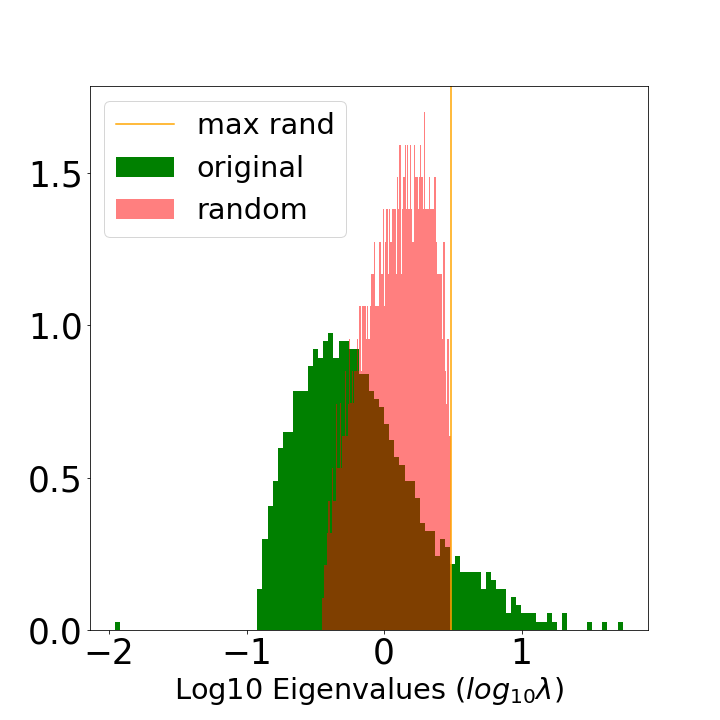
\includegraphics[width=7cm]{./img/shape-scale-a.png}
      \label{fig:scale-shape-a}
    }                               
    \subfigure[ESD with \CorrelationTrap]{                   
      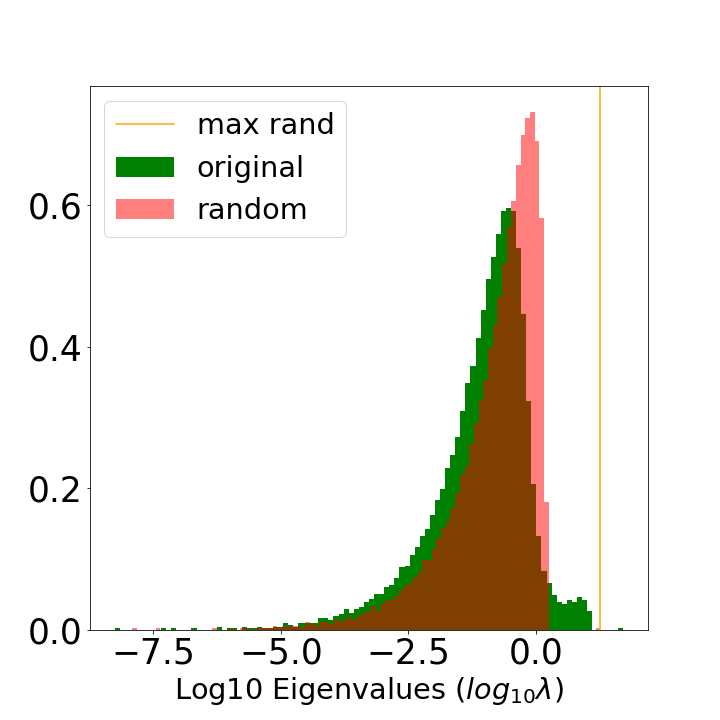
\includegraphics[width=7cm]{./img/shape-scale-b.png}
      \label{fig:scale-shape-b}                           
    }                                                                                                                            
    \caption{Comparison of a well-formed, Heavy-Tailed ESD (a) to one with a Correlation Trap (b), in the VGG16 model (FC2 layer)}
  \label{fig:scale-shape}                                                                                                      
\end{figure}

See Figure~\ref{fig:scale-shape-a}, which displays the (log)-ESD of a \Typical SOTA NN layer $\mathbf{X}$ (green), i.e., on a log-linear scale, along with the (log)-ESD of that layer after randomizing it element-wise (red).
The two ESDs differ substantially:
the ESD of the original weight matrix  $\mathbf{W}$ (green) is very HT, whereas 
the ESD of the randomized weight matrix  $\mathbf{W}^{rand}$ (red) is an MP (and as predicted by the MP \RMT).
The orange line corresponds to the maximum eigenvalue of the randomized ESD.
Note that it is at the MP bulk edge of the red plot, indicating that this ESD is not affected by unusually large elements or other weight anomalies.
Here, we say that the ESD of $\mathbf{X}$ is HT, and that $\mathbf{W}$ is not HT element-wise.
\HTSR says this layer is well trained.

Contrast this with Figure~\ref{fig:scale-shape-b}, which displays the (log)-ESD of a NN layer with a \CorrelationTrap.
The ESD of $\mathbf{X}$ (green) is weakly HT, but it looks nothing like the ESD in Figure~\ref{fig:scale-shape-a}.
In fact, it looks very much like the ESD of the randomized weight matrix  $\mathbf{W}^{rand}$ (red), except for a small shelf on the right. 
The orange line again corresponds to the maximum eigenvalue of the randomized ESD, and this is just past this shelf.
Relative to the randomized ESD, this line depicts (an) unusually large element(s)---or, equivalently, a rank-1 perturbation of $\mathbf{W}^{rand}$.
By a \CorrelationTrap, we mean that some anomaly in the elements of $\mathbf{W}$ tends to ``trap'' the ESD of $\mathbf{X}$, concentrating the correlations in $\mathbf{X}$ into the small shelf of density around the orange line. 
\HTSR says this layer is not well-trained because it does not have a good PL fit.

%We will see, below in Section~\ref{sxn:empirical}, that we can induce a \CorrelationTrap by shrinking the batch size, and that this is associated with a degradation in model performance (%as well as spuriously low PL exponent $\alpha$). 


%\paragraph{Correcting for \SCALE Anomalies with \ALPHAHAT}
%\subsubsection{Correcting for Scale Anomalies with \ALPHAHAT}

%\nred{repetitive ?}
%  \CorrelationTraps are a kind of \SCALE anamoly;by this we mean when the layer weight matrix $\mathbf{W}$
%  and/or the randomized  $\mathbf{W}^{rand}$ has one or more unusually large eigenvalues $\lambda$.
%  In the case of a scale anamoly, the simple PL \ALPHA metric may not correlate well with the test accuracy or other measures
%  of model quality because such scale anomalies may make it difficult to get a good PL fit of $\alpha$.
%  In some very hard cases, the layer ESD $\rho_{emp}(\lambda)$ may be significantly deformed from a well
%  behaved PL or TPL distribution (as in Fig.~\ref{fig:scale-shape-b}.  In these cases, the \ALPHAHAT
%  metric can frequently compensate.  This is seen in Section~\ref{sxn:empirical} \nred{see github issue 46}

 





\subsubsection{Over-Regularization}
\label{sxn:underfitting}

%\michael{Is the idea that this section parallels Section~\ref{sxn:Traps}, in that both describe non-\Ideal learning?  If so, we need to refine.  Are we saying that the primarily way $\alpha<2$ is when one layer is compensating for another.  }

The second way we identify $\mathbf{W}$ as \ATypical is when it has an anomalously large variance $(\sigma^2(\WMAT))$.
\michaeladdressed{Variance of what.}

The \SETOL theory -- a single-layer theory of learning -- casts the training 
of a NN layer in terms of how the correlations concentrate into the layer  \EffectiveCorrelationSpace (\ECS),
and becomes exact when the \TRACELOG condition is satisfied.
Analogously, the \HTSR theory -- a single layer \Phenomenology of learning -- casts training
of an N layer by fitting its ESD to a PL, and noting that the PL exponent $\alpha$ measures
the amount of implicit regularization in the layer.
Comparing the two approaches, we see that smaller $\alpha$ corresponds to the correlations
concentrating into a low-rank~\ECS.  In general, and likewise, the more the weight matrix
correlations concentrate  into a low-rank~\ECS, the better the layer has been regularized.
A natural question arises then, namely, can a layer be \emph{\OverRegularized} and
can we detect this?
and in large,
Empirically, we do indeed observe that over the course of training, $\alpha$ decreases, (See Figure~\ref{fig:mlp3-FC1-alpha-overloaded} 
(a), Section~\ref{sxn:hysteresis_effect},) and that the models predictions are concentrated into the~\ECS, 
(See Section~\ref{sxn:empirical-effective_corr_space}). Thus, we also interpret $\alpha$ and~\ECS concentration to be 
measures of learning itself, meaning that NNs are self-regularizing~\cite{MM18_TR_JMLRversion}.

Importantly, however, the \HTSR \Phenomenology indicates that \ALPHA usually lies in the Fat-Tailed Universality class,
such that $\alpha\in [2,6]$.  When $\alpha <2$, the ESD is Very Heavy Tailed (VHT), and, also,
this indicates that $\mathbf{W}$ has an anomalously large variance.  That is,  $\mathbf{W}$ is  \ATypical.
Occasionally, but very infrequently, we do observe $\alpha<2$, and in large, production quality models
(like Llama).
Interestingly, we also observe that, frequently, when the \HTSR $\alpha<2$, the \SETOL \TRACELOG
condition holds fairly well.  This is further explored in Section~\ref{sxn:empirical}

We have applied the \WW tool to have examined dozens
of modern, very large NNs; of particular interest are the so-called Large Language Models
(LLMs) that have revolutionized the field of AI.  To that end, in Figure.~\ref{fig:falcon_vs_llama},
we present the \WW layer \ALPHA metrics for the Falcon-40b and the Llama-65b LLMs.
\footnote{Similar results are found for the larger, more modern Llama models,
and can be found on the ~\WW website\cite{WW}}

\begin{figure}[ht!]
    \centering
    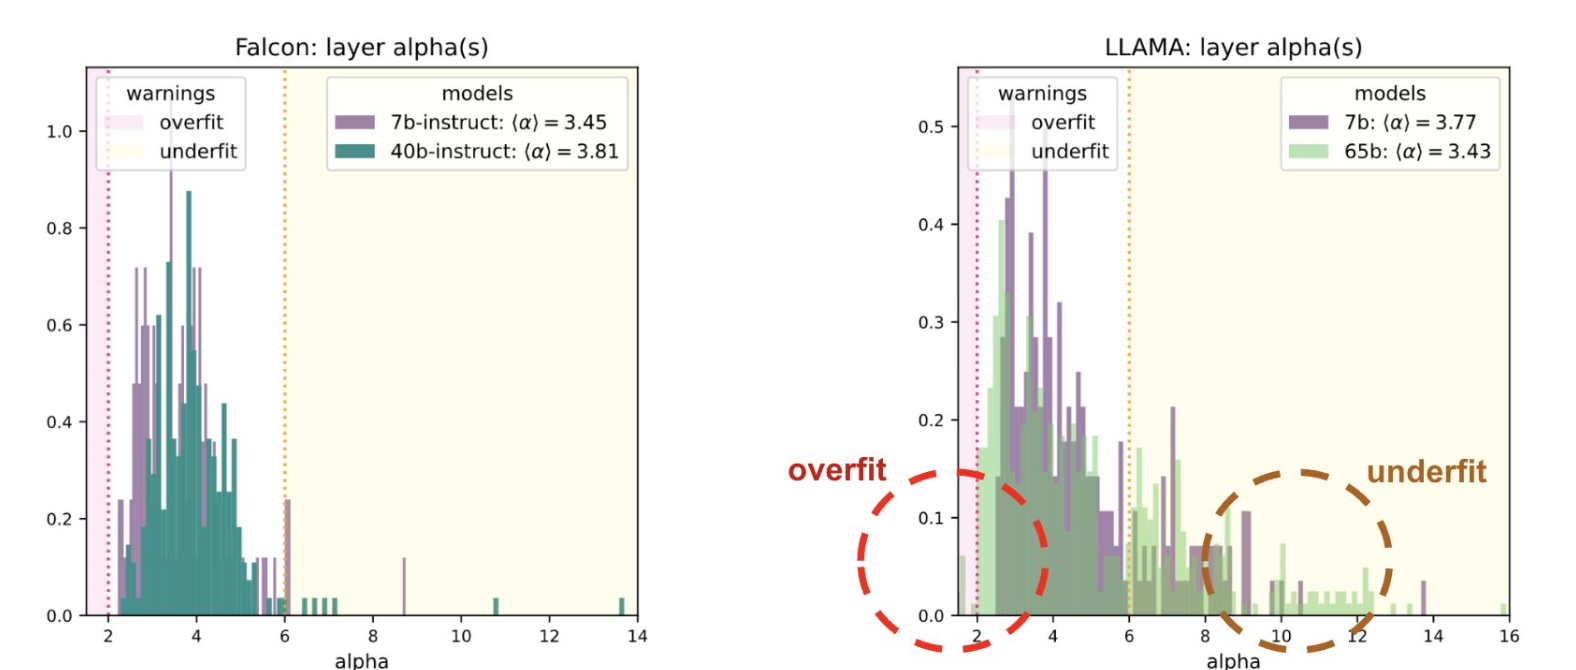
\includegraphics[width=15cm]{./img/falcon_vs_llama.png}
    \caption{Falcon vs Llama}
   \label{fig:falcon_vs_llama}
\end{figure}

For the Falcon-40b model, all of the layer \ALPHA range between $\alpha\in[2,6]$,
and therefore lie in the Fat-Tailed Universality class (in Table~\ref{tab:Uclass})
and are well-fit.
In contrast, looking at the Llama-40b layer \ALPHA, very many have $\alpha>6$,
indicating these layers are under-fit, and while a few have $\alpha <2$, suggesting
these are over-fit.  Finally, there are more layers with $\alpha~\sim2$ in Llama-65
vs Falcon-40b.

The observations on Llama-2 suggest that the layers with $\alpha\le 2$
are compensating for the layers with $\alpha>6$, and yielding suboptimal
performance for the Llama-65b architecture.
Based on these observations, we hypothesize that, in a multi-layer-perceptron (MLP),
when one layer does not or can not learn, then other layers will
have to compensate, and will be overloaded with the training data,
leading to $\alpha<2$, and even the \TRACELOG condition $\Delta \lambda_{min} < 0$.

%In Section~\ref{sxn:empirical} below, we will test this hypothesis in a 3-layer MLP model
%(MLP3), trained on MNIST, but only training 1 (FC1 or FC2), while keeping the other 2 frozen.
%In this way, we can simulate the situation seen above in the Llama-65b model,
%and observe the formation of a VHT ESD in the layer being trained.

%Additionally, as argued below, we conjecture that when $\alpha<2$, the model
%enters a kind-of glassy meta-stable phase, similar to the kinds of phases
%predicted by classic \STATMECH theories of learning.  A
%\nred{explain idea that VHT is \ATypical}

%We will explore how far we can push this analogy in our experiments to stress test the \SETOL approach.
%In particular, we will see effects reminiscent of a glassy system-the slowing down
%of the dynamics (in Sections~\ref{sxn:fc1})
%and a kind of hysteresis (Section~\ref{sxn:hysteresis_effect})

In Section~\ref{sxn:hysteresis_effect}, we will test this hypothesis.
By reducing the trainable parameters in a small MLP, we can simulate the situation seen above in the Llama-65b model,
and observe the formation of a Very Heavy Tailed (VHT) ESD in the dominating layer weight matrix.
Overloading results from having too few parameters for the complexity of the task. Adding more data increases 
the load up to the total complexity of the task itself.
%\st{Adding noisy labels increases the load up to the capacity of the a}

Moreover, we will also argue that in our experiments,
the model enters a kind of glassy meta-stable  phase, similar to the kinds of phases predicted by
classic \STATMECH theories of learning~\cite{SST92}
(described below).
Section~\ref{sxn:hysteresis_effect} will explore how far we can push the analogy of glassy systems in our experiments to 
stress test the \SETOL approach. In particular, we will see effects such as the slowing down of its dynamics, leading to a kind 
of hysteresis, specific to the under-parameterized regime.





